\documentclass[conference]{IEEEtran}

\usepackage{cite}
\usepackage{graphicx}
\usepackage{tabularx, booktabs}
\hyphenation{op-tical net-works semi-conduc-tor}

\begin{document}

\title{Performance Analysis of CNN Frameworks\\for GPUs}

\author{\IEEEauthorblockN{HeeHoon Kim}
\IEEEauthorblockA{Department of Computer Science and Engineering,\\
Seoul National University, Korea\\
Email: hydrogen@snu.ac.kr}
\and
\IEEEauthorblockN{Hyoungwook Nam}
\IEEEauthorblockA{Department of Computer Science and Engineering,\\
Seoul National University, Korea\\
Email: hwnam831@snu.ac.kr}}

\maketitle

\begin{abstract}
Convolutional neural network has been successful in visual recognition tasks.
Machine learning frameworks are using GPU deep learning libraries to efficiently implement CNNs on GPUs.
This study analyzes GPU performance characteristics of Theano, Caffe, Torch and Tensorflow via benchmarking AlexNet model on them.
The GPU utilization and framework overheads are analyzed and we suggest possible optimization methods to increase efficiency.
We also identify differences between 4 convolution algorithm kernels - GEMM, direct, FFT and Winograd convolution.
Layerwise comparison and analysis show performance characteristics of the kernels.
We suggest criterions for choosing convolution kernels and methods to create efficient CNN model on the GPU.
As scaling DNN on multi-gpu context becomes important, we compare data parallelism implementations of the frameworks.
Scalability and synchronization overheads are analyzed.
We suggest possible methods to improve multi-gpu scalability of the frameworks.
Also we provide methods to build scalable DNN model on multi-gpu context.

\end{abstract}

\IEEEpeerreviewmaketitle


\section{Introduction}

Deep neural networks(DNN) have been very successful on various machine learning tasks such as visual recognition, speech recognition and machine translation.
Convolutional neural network(CNN), proposed by LeCun et. al., is one of the earliest successful neural network model used for image classification tasks.
\cite{726791}%% lenet
CNN with Deep learning methods (e.g. ReLU activation, Dropout layer, Data augumentation) outperformed previous machine learining methods on visual recognition challenge.
\cite{DBLP:journals/corr/RussakovskyDSKSMHKKBBF14}%% alexnet, googlenet, VGG
Classification accuracy of CNN models have been improving over time and recent state-of-the-art programs for visual recognition use ensemble of CNN models.
\cite{ILSVRC15}%% ILSVRC 2016 winner
CNN models are also being applied to other machine learning tasks other than image recognition. CNN can be applied to action recognition, speech recognition, natural language processing and AI playing game of Go.
\cite{6857341, cite-key , DBLP:journals/corr/KalchbrennerGB14}%% one of each

The biggest advantage of applying DNN is its scalability, means that larger and deeper DNN with more input data usually results in better accuracy.
Bigger DNN requires more processing power, hence training DNN by typical computer is impractical.
Luckily, computations in neural network can easily be represented as tensor or matrix operations, which can be efficiently parallelized.
Therefore, Grahpics Processing Unit(GPU)'s parallel processing power made DNN possible to train on single machine.
Deep learning frameworks have been developed for easy and efficient implementation of DNN models, and most popular frameworks support GPU acceleration by default.
\cite{DBLP:journals/corr/Al-RfouAAa16,jia2014caffe,tensorflow2015-whitepaper,torch, cntk} 
Companies and researchers have been trying to implement efficient GPU kernels to improve performance.
The most popular one is CuDNN, a GPU deep learning library created by NVIDIA that has been adopted as GPU-backend of popular frameworks.
\cite{cudnn} %% CuDNN
Convolution with CuDNN results in up to 4x performance improvement from default GPU kernels of the frameworks.
\cite{convnet-benchmarks} %% convnet-benchmark
The another approach to speed up CNN is reducing time complexity of convolution algorithm.
Fast Fourier transform(FFT) algorithm and Winograd's minimal filtering algorithm successfully reduced algorithm complexity of convolution.
\cite{fftconv, winograd, fbfft} %% fft and winograd
Efficiency of deep learning on single GPU has been improved a lot, while deep learning on multiple GPU still showing poor scalability.
\cite{DBLP:journals/corr/YadanATR13} %% model parallelism, distributed deep learning


In this study, we analyze GPU performance characteristics of convolutional neural network on different frameworks or libraries.
For disambiguation, in this paper the word 'framework' refers to a full collection of libraries to build DNN models, and the word 'library' refers to a GPU kernel library for DNN.
We choose 4 most popular deep learning frameworks, Theano, Caffe, Torch and TensorFlow by the number of github stars.
The popular CNN model for benchmarking purpose is AlexNet model.
\cite{krizhevsky2012imagenet}
The identically structured AlexNet models are built and trained on the frameworks.
All 4 frameworks use CuDNN as GPU backend library.
Cuda-convnet is another GPU library developed by Alex Krizhevsky of AlexNet.
\cite{cuda-convnet}
3 different convolution algorithms of CuDNN are compared with direct convolution algorithm of Cuda-convnet.

The analysis experiments can be divided into 3 parts.
The first part of the experiments compares differences in performance characteristics of the frameworks.
The comparison would provide detailed pros and cons of deep learning frameworks to propspect users.
Also performance limiters identified from this study would help framework developers to optimize the frameworks.
The second part of the experiments take a close look into GPU kernels to analyze performance characteristics of different convolution algorithms.
Based on the analysis, we provide optimization methods to implement efficient CNN model using the GPU deep learning libraries.
The final part analyzes performance characteristics of the frameworks on multi-gpu context.
Discussion section would contain possible methods to improve multi-gpu scalability.

\section{Background and Related work}

\subsection{Previous work}
It has been only a few years since deep learning frameworks were introduced to public.
Few attempts recently tried to benchmark and compare the performance of the frameworks.
A benchmark of CNN frameworks is publicly available on Github.
\cite{convnet-benchmarks}.
It shows forward and backward propagation time of CNN model for each framework.
But the latest result was tested with cuDNN version R4, while the most recent version is R5.1.
Detailed benchmarks of deep learning frameworks were recently published.
\cite{DBLP:journals/corr/BahrampourRSS15, DBLP:journals/corr/ShiWXC16}
They show execution times of various DNN models run on the frameworks.
However, the benchmarks show only the results, without identifying the reasons for the differences.
They also use cuDNN version of R4, which do not support most recent Winograd convolution.


\subsection{Machine learning frameworks}

Theano is a python framework for evaluating mathematical expressions. 
\cite{DBLP:journals/corr/Al-RfouAAa16}
It is one of the earliest framework used to build DNN models such as Deep Belief Network.
Multiple machine learning frameworks are built on top of Theano.
Keras and Lasagne are popular frameworks for DNN using Theano as their backend.
Multiple GPU support of Theano is still on experimental stage.
Torch is a scientific computing framework based on Lua language.
\cite{torch}
Torch is also one of the earliest frameworks used to implement CNN models.
Nvidia's self driving car project and Deepmind's Deep Q Learning model were built on Torch.
\cite{nvdave, mnih2015humanlevel}
Torch natively supports multi-gpu context via its cutorch module.
Caffe is deep learning framework developed by Berkeley Vision and Learning Center.
\cite{jia2014caffe}
Caffe use prototxt file to describe DNN models.
Pre-trained network models can be imported with prototxt files.
Visual recognition challenge winners are usually implemented by Caffe.
\cite{ILSVRC15, RCNN, vgg}
The flexibility of Caffe is limited.
Introducing a new feature to a layer requires re-building of the entire source code.
The multi-gpu support of Caffe is limited to batch data parallelism.
Tensorflow is machine learning framework developed by Google.
\cite{tensorflow2015-whitepaper}
It was first introduced to public in 2015, and is now the most popular machine learning framework on GitHub.
Tensorflow supports both Python and C++ interface.
Computational Network Toolkit(CNTK) is deep learning framework developed by Microsoft.
\cite{cntk}
CNTK supports both Windows and Linux environment, while the others do not support Windows.
CNTK uses its own BrainScript to describe DNN models.
It also supports C++ and C\# wrappers to evaluate models.

\begin{figure}
  \centering
  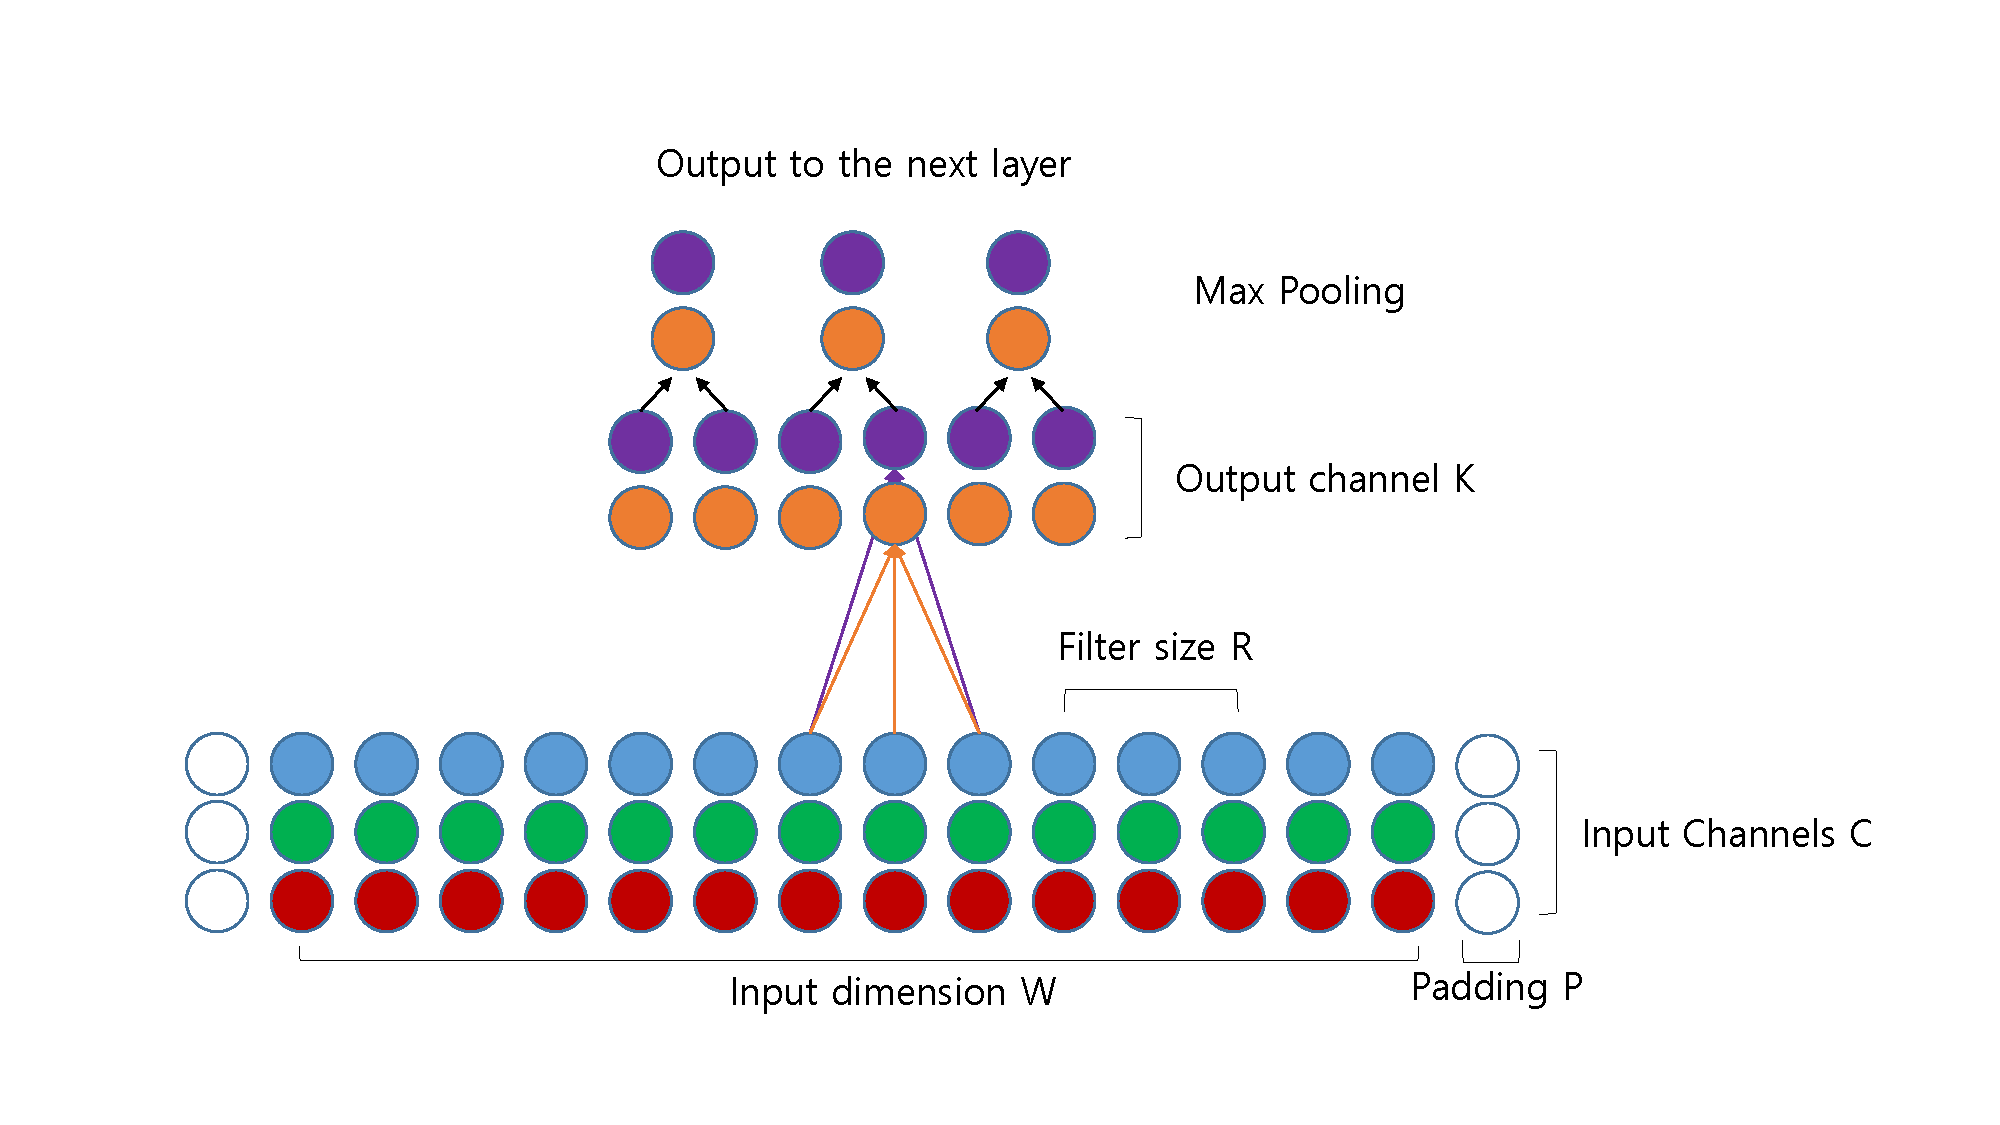
\includegraphics[width=\linewidth]{./figures/convlayer}
  \caption{An example of typical 1D convolution. K filters of filter size R convolves among input of dimension W with C channels.
	Each convolutional filter becomes an output channel. Pooled output feature map is fed to the next layer. }
  \label{fig_convlayer}
\end{figure}

\subsection{Convolutional Neural Network}
Convolutional Neural Network(CNN) is an Artificial Neural Network using convolutional filter to extract features from input.
Figure \ref{fig_convlayer} shows an example of 1D convolutional layer.
K filters of filter size R convolves among input data of dimension W.
Each convolutional filter activation corresponds to a channel of output feature map.
A nonlinear activation function is applied to calculate an activation of a filter.
Typical CNN uses Rectified Linear Unit(ReLU) for nonlinear activation.
A convolution by stride S and padding P creates a feature map of dimension (W - R + P + 1)/S with K channels.
Usually a pooling layer is applied to reduce the output dimension.
The 2D spatial convolution as input dimension of W*W and kernel size of R*R creating feature map of dimension ((W-R+P+1)/S)\^2.
The computational complexity of propagating such convolutional layer is O(K * CRR * WW).

\subsection{Convolution algorithms}
Several methods are used to efficiently implement convolution on GPU.
Direct convolution is the most straightforward way but needs a lot of specialized kernels to optimize for various input dimensions and corner cases.
Cuda-convnet \cite{cuda-convnet} is the efficient direct convolution library written by Alex Krizhevsky, the author of AlexNet paper.
CuDNN however, treats convolution as matrix multiplication(GEMM) \cite{cudnn}.
The convolution layer of K kernels with dimension R*R and W*W input with C channels is converted to multiplication of K*CRR filter matrix and CRR*NWW data matrix.
The dimensions of matrices are very big, hence the multiplication can be parallelized using highly efficient BLAS libraries.
Converting convolution to matrix might require significant amount of memory bandwidth.
CuDNN computes the multiplication by tiles to hide memory latency while computing.
This method scales well on small batch sizes and can be used on all types of convolution layers.
The complexity of both methods are basically the same.

FFT convolution uses fast Fourier transform algorithm to reduce algorithm complexity \cite{fftconv}.
Typical convolution has algorithm complexity of O(K * CRR * WW), while FFT convolution shows complexity of O(K * CWW * log(W)) which does not depend on the size of the filter.
FFT convolution requires more memory space since filters must be padded to the dimension of inputs.
However, FFT convolution cannot be applied to convolution with stride more than 1.
Winograd convolution algorithm is based on GEMM convolution but reduces algorithm complexity using Winograd's minimal filtering algorithm.
Using Winograd’s minimal filtering algorithm, matrix multiplication of 4x3 tiled matrix requires 6 multiplications instead of 12.
Nesting the minimal filtering algorithm reduces 12*12 multiplications into 6*6 multiplications, reducing algorithm complexity by 4\cite{winograd}.
However, different sized kernel needs its own minimal filtering algorithm, hence CuDNN 5.0 only supports Winograd convolution for filter size of 3x3.

\subsection{Multi-gpu parallelism}
Multi-gpu implementation of deep neural networks can be implemented by data parallelism or model parallelism \cite{NIPS2012_4687}.
On data parallelism, a batch of inputs is divided and distributed among devices.
After backpropagation, the entire gradients of network parameters must be passed to single device in order to compute stochastic gradient descent.
And then the updated parameters are distributed among devices.
Hence, the communication cost of data parallelism depends on number of parameters in the network.
AlexNet has 65M parameters, thus each iteration needs to transfer approximately 520MB of data per GPU.
On the other hand, model parallelism divides and distributes the network on each GPU.
Since parameter updates can be done on each GPU, only a small amount of activation data is communicated between GPU.
Carefully designed model parallelism of convolution layer outperforms the data parallelism \cite{DBLP:journals/corr/YadanATR13}.
However, multi-gpu support on Caffe is limited to data parallelism, therefore we only compare data parallelism efficiencies of the frameworks.
Tensorflow and Torch supports both data and model parallelism while Theano doesn’t support multi-gpu natively.

\section{Experiment setup}

\subsection{System setup}
We test the frameworks on the CentOS 7.2 server with 4 octa-core Xeon-E5 cpus and 4 GTX TITAN X(GM200) gpus.
We use Cuda 7.5 and CuDNN R5 which is the latest stable release of Cuda and CuDNN.
All deep learning frameworks are updated to latest stable release on June 2016.
The versions of the frameworks fully support CuDNN R5.
Only Torch supports the latest version of Cuda-convnet3.
The detailed system environments are represented on Table \ref{} and \ref{}.

CentOS 7.2.1511 / Linux 3.10.0-327 / Inte Xeon E5-2650@2.0GHz / 128GB DDR3@1600MHz / CuDNN 5005 / Cuda 7.5 / Torch 7 ccn2.torch, cudnn.torch R5 / Theano 0.8.2 / Caffe * / Tensorflow *
%TODO

\subsection{AlexNet model}
AlexNet \cite{krizhevsky2012imagenet} is one of the earliest successful deep neural networks on image recognition task using ImageNet dataset.
AlexNet uses 5 convolution layers to extract features and 3 fully connected layers for classification.
Each layer has rectified linear unit(ReLU) layer for nonlinear activation.
AlexNet has been frequently used for benchmarking performance of machine learning libraries, because it utilizes most of the current DNN components such as convolution, max-pooling and dropout.
The original AlexNet model includes Local response normalization(LRN) layer, but we exclude it for benchmarking task since LRN is very rarely used in current convolutional neural networks.
The detailed layer structure of AlexNet model on this study is presented in Table \ref{alex_model}.


\begin{table*}[]
\centering
\caption{Alexnet model used on benchmarking}
\label{alex_model}
\begin{tabular}{llllllll}
Name    & Kernel(R) & Input Channels(C) & Ouput Channels(K) & Stride(K) & Sample width(W) & Params & Flop \\
Input   &           & 3                 &                   &           & 227 x 227       &        &      \\
Conv1   & 11 x 11   & 3                 & 96                & 4         & 55 x 55         & 35K    & 55G  \\
Pool    & 3 x 3     &                   &                   & 2         &                 &        &      \\
Conv2   & 5 x 5     & 96                & 256               & 1         & 27 x 27         & 614K   & 227G \\
Pool    & 3 x 3     &                   &                   & 2         &                 &        &      \\
Conv3   & 3 x 3     & 256               & 384               & 1         & 13 x 13         & 885K   & 65G  \\
Conv4   & 3 x 3     & 384               & 384               & 1         & 13 x 13         & 1.3M   & 98G  \\
Conv5   & 3 x 3     & 384               & 256               & 1         & 13 x 13         & 885K   & 65G  \\
Pool    & 3 x 3     &                   &                   & 2         &                 &        &      \\
FC6     &           & 256 x 6 x 6       & 4096              &           &                 & 37M    & 74M  \\
FC7     &           & 4096              & 4096              &           &                 & 16M    & 32M  \\
FC8     &           & 4096              & 1000              &           &                 & 4M     & 8M   \\
Softmax &           & 1000              & 1000              &           &                 &        &     
\end{tabular}
\end{table*}


\section{Results/Analysis}

\subsection{Single GPU analysis}


\subsection{characterization of different convolution algorithms}
Since forward and backward propagation of convolution layers takes most of the running time, we run the same model on different convolution kernel to characterize the performance of each convolution algorithm.
Three types of convolutions are computed for each iteration.
forward convolution(FWD) computes the layer output, backward data convolution(BD) computes backward gradient input and backward filter convolution(BW) computes gradients of network parameters.
CuDNN R5 supports matrix multiplication convolution(gemm), FFT convolution, and winograd convolution.
CuDNN has various gemm convolution algorithms and the tested algorithm is implicit gemm precomp algorithm.
Winograd convolution cannot be applied to BW convolution on CuDNN 5.0 hence we use fft convolution instead.(CuDNN 5.1RC supports winograd nonfused option)
Since the first convolution layer has stride of 4, Winograd and FFT convolution cannot be applied.
Direct convolution is tested by Torch binding of Cuda-convnet3.
All comparisons are done on Torch 7 because Torch can specify convolution algorithm on each layer and newest version of Cuda-convnet3 is only supported by Torch7.

Randomly generated batch inputs are used to remove IO latency.
The forward and backward propagation time is measured as average of 100 iterations.
The compute times and statistics of kernels are measured by NVIDIA nvprof profiler.
The theoretical floating point operation counts are calculated as 2 * (batch size) * K*CRR*WW since each calculation uses 1 addition and 1 multiplication.
We compare them to actual floating-point operation counts of the kernels.
Flops of the kernels are calculated as Flop count/execution time.
FFT convolution consists of 2 FFTs and 1 complex matrix multiplication, thus statistics of those 3 kernels are added together.

\begin{figure}
  \centering
  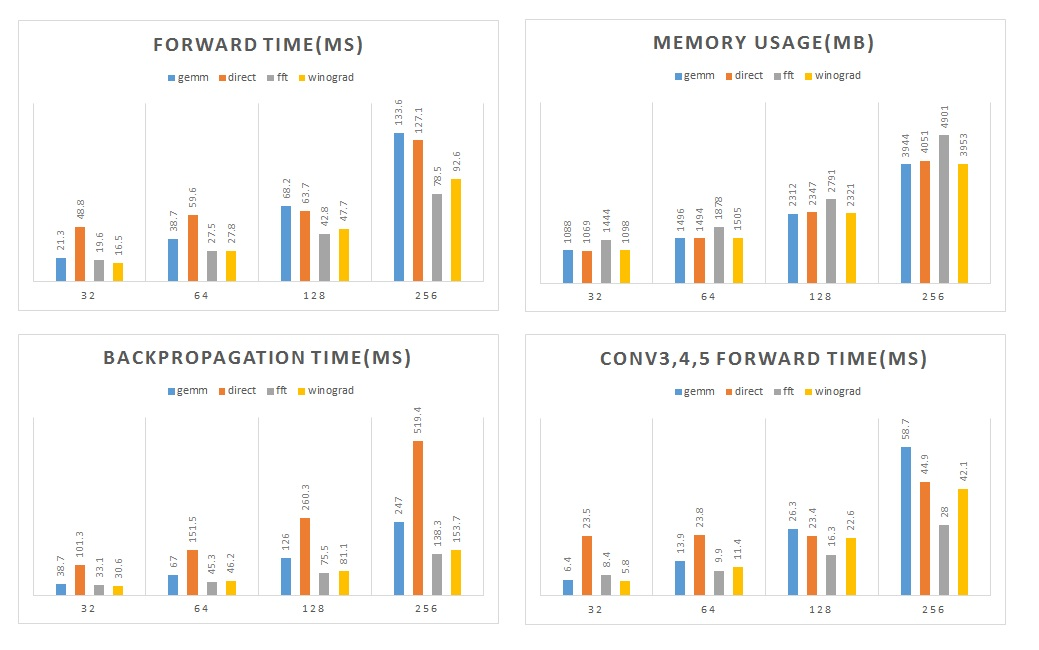
\includegraphics[width=\linewidth]{./figures/conv_time}
  \caption{Forward propagation and Backpropagation times of convolution algorithms. The times are measured as average of 100 batch iterations. 
Direct convolution is tested with cuda-convnet3 and other 3 are kernels of CuDNN R5. }
  \label{fig_conv_time}
\end{figure}

FIg \ref{fig_conv_time} shows execution time comparisons between convolution kernels.
Winograd convolution and FFT convolution always perform better than direct or gemm convolution, due to smaller floating point operations required.
FFT has smallest operations count, makes it fastest among algorithms on big batch inputs.
However FFT scales bad on smaller batch sizes because it executes 5 kernels per each layer.
The forward propagation speed comparison on conv layer 3,4,5 on (f) of Fig \ref{fig_conv_time} clearly shows the differences.
Cuda-convnet scales bad when the batch size is smaller than 128 while GEMM convolutoin sclaes almost linearly.
Winograd performs better when the batch size is smaller than 64, where theoretical operations per each layer is around 20G operations.
Winograd kernels are more efficient when the sample width is even.
When we increase the sample width of conv layer 3,4,5 from 13 to 14, the execution time of Winograd kernels decrease by 10\%.

Number of floating point operations needed for forward propagation and backward propagation kernels are equal on the same layer.
Therefore, execution time of forward and backward propagation kernels are almost symmetric on most convolution algorithms.
However, backpropagation kernels of direct convolution takes more execution time than their forward counterparts.
Especially backward filter convolution on first convolution layer takes 200ms to execute, occupying 40\% of total training time.
The reason for the slow execution is low parallelism of kernels.
The backward direct convolution kernels have small thread numbers compared to other algorithms, generating 6 times smaller thread grid size.
The backward filter convolution for the first layer generates only 1024 threads, while Titan X has 3072 CUDA cores.





\begin{figure}
  \centering
  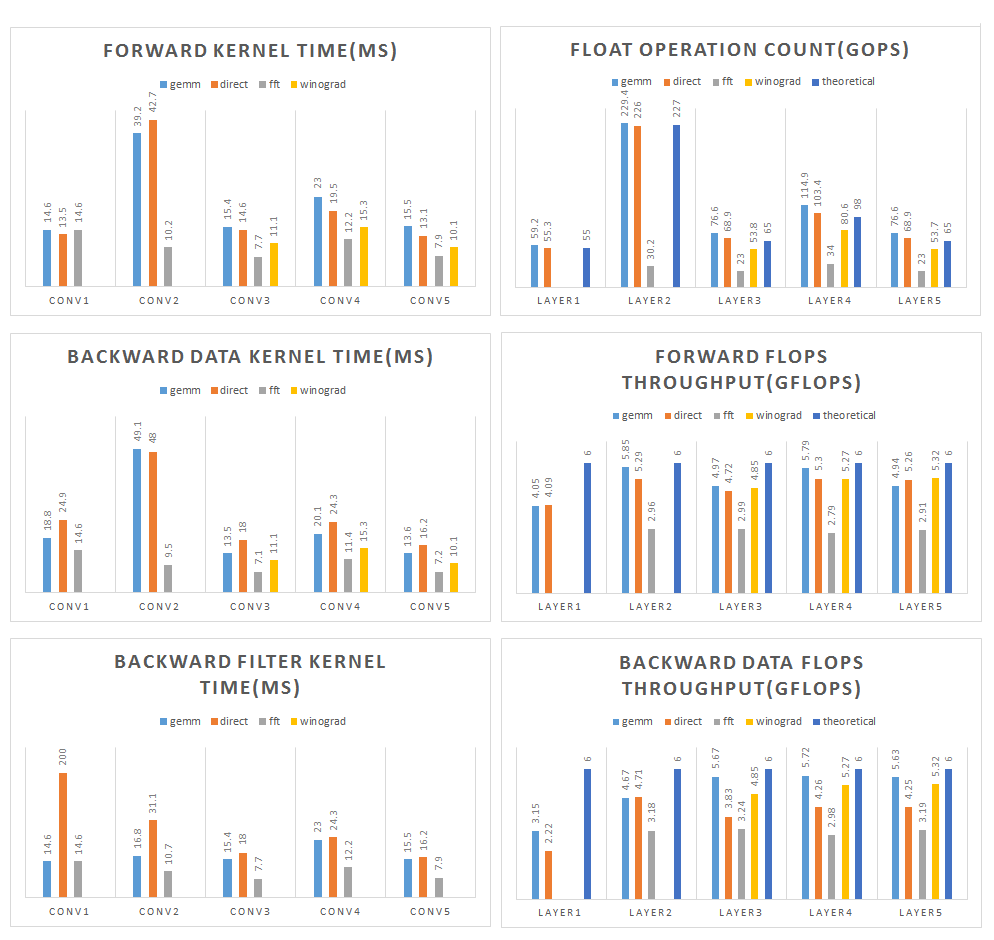
\includegraphics[width=\linewidth]{./figures/layerwise_bench}
  \caption{Layerwise analysis of convolution kernels}
  \label{fig_layerwise}
\end{figure}


\subsection{Multi GPU analysis}

\begin{itemize}
  \item Support
  \item Scalability : proportion of data exchange
  \item Synchronization cost
\end{itemize}

\section{Discussion / Conclusion}

\begin{itemize}
  \item Summary of results
  \item Compare frameworks : Implementation difference
  \item Locate bottleneck / suggest possible optimization
  \item Limitation, future research
\end{itemize}

\section*{Acknowledgment}

The authors would like to thank...

\bibliographystyle{IEEEtran}
\bibliography{IEEEabrv,PACFG}
\nocite{*}

\end{document}
